\documentclass[aspectratio=169,
				xcolor=table]{beamer}
				
% Load general definitions
\usepackage[utf8]{inputenc}
%\usepackage[T1]{fontenc}
\usepackage[brazil]{babel}
\usepackage{amsmath}
\usepackage{amsfonts}
\usepackage{amssymb}
\usepackage{graphicx}
\usepackage{verbatim}
\usepackage{cancel}
\usepackage{askmaps}
\usepackage{tabularx}
\usepackage[table]{xcolor}
%\usepackage{tikz}
\usepackage{multirow}
\usepackage{mathtools}
\usepackage{color, colortbl}
\usepackage{etoolbox}
\usepackage{pbox}
\usepackage{changepage}
\usepackage{xpatch}
\usepackage{array}
\usepackage{marvosym}
\usepackage{tabu}
\usepackage{multicol}
\usepackage{listings}
\usepackage{underscore}
\usepackage{filecontents}
\usepackage[]{algorithm2e}
\usepackage{ragged2e}

\newcolumntype{P}[1]{>{\centering\arraybackslash}m{#1}}
\definecolor{Gray}{gray}{0.75}
\definecolor{Gray2}{gray}{0.85}

\definecolor{lightBlue}{HTML}{DAE8FC}
\definecolor{Blue}{RGB}{51, 51, 204}

%\useinnertheme[lily]{rounded}
\usetheme{UniEvangelica}
%\usetheme{Copenhagen}
%\usetheme{Berlin}
%\usecolortheme{dolphin}
\tolerance=1
\emergencystretch=\maxdimen
\hyphenpenalty=10000
\hbadness=10000

\setbeamertemplate{navigation symbols}{}%remove navigation symbols


\let\olditem=\item% 
\renewcommand{\item}{\olditem \justifying}%
\def\center{\trivlist \centering\item\relax}
\def\endcenter{\endtrivlist}

\setbeamertemplate{itemize/enumerate body begin}{\large}
\setbeamertemplate{itemize/enumerate subbody begin}{\large}

\setbeamertemplate{itemize item}{\raisebox{0.1ex}{$\blacktriangleright$}\hskip0.1em}
\setbeamertemplate{itemize subitem}{\raisebox{0.1ex}{$\blacktriangleright$}\hskip0.1em}

\newcommand{\greenarrow}{\textcolor{green}{\rotatebox[origin=c]{180}{\MVArrowDown}}}

\newcommand{\redarrow}{\textcolor{red}{\MVArrowDown}}

%\newcommand{\ftable}{
%	\begin{table}
%		\large
%		\centering
%		\rowcolors{1}{\ifnumless{\rownum}{2}{Blue}{lightBlue}}{}
%}

\newenvironment{eftable}{
	\begin{table}
		\large
		\centering
		\rowcolors{1}{}{Blue}
		\rowcolors{1}{\ifnumless{\rownum}{2}{Blue}{lightBlue}}{}
	}
	{
	\end{table}
}


%\setbeamertemplate{frametitle}
%{
%	%\vspace*{-2em}	
%	\insertframetitle
%
%	 %\textcolor{white}{\LARGE \insertframetitle}
%
%}

% Specific definitions
\institute[]{\uppercase{Engenharia de Software}}
\title[]{Arquitetura e Organização de Computadores}
\subtitle[]{\uppercase{Barramentos}}
\author[]{Prof. Alexandre Tannus}
\date{}

\AtBeginSection{\frame{\tableofcontents[currentsection]}}

\begin{document}

	\begin{frame}
		\titlepage
	\end{frame}

	\begin{frame}{Objetivos}
		\begin{itemize}
			\item Explicar o funcionamento de um barramento
			\vspace{1em}
			\item Classificar barramentos quanto ao tipo, método de arbitração, sincronização e tipo de transferência de dados
			\vspace{1em} 
			\item Examinar os diferentes tipos de barramentos existentes
		\end{itemize}
	\end{frame}

	\begin{frame}{Metodologia}
		\begin{itemize}
			\item O tema da aula é exposto pelo professor em sala de aula. Os alunos interagem durante a apresentação para resolução de dúvidas e exposição de questionamentos relevantes ao tema, os quais podem ser sanados diretamente pelo professor ou serem colocados em discussão pela turma. 
			\vspace{1em}
			\item Ao final da exposição do conteúdo são resolvidos exercícios de fixação, para melhor compreensão do tema. As questões podem ser retiradas de concursos públicos, ENADE, POSCOMP ou de autoria do próprio professor.
		\end{itemize}
	\end{frame}

	\begin{frame}
		\tableofcontents		
	\end{frame}	
	
	\section{Introdução}
	\begin{frame}
		\frametitle{Introdução}
		\begin{itemize}
			\item O computador é um conjunto de componentes de três tipos básicos
			\begin{itemize}
				\item Processador
				\item Memória
				\item Entrada/Saída
			\end{itemize}
			\vspace{1em}
			\item Estrutura de interconexão
			\begin{itemize}
				\item Caminhos que conectam os componentes
				\item Projeto depende das trocas que precisam ser efetuadas entre os módulos
			\end{itemize}
		\end{itemize}
	\end{frame}
	
	\begin{frame}
		\frametitle{Estrutura de interconexão}
		\framesubtitle{Tipos de transferência}
		\begin{itemize}
			\item Processador $\Leftrightarrow$  memória
			\vspace{1em}
			\item Processador $\Leftrightarrow$  E/S
			\vspace{1em}
			\item E/S $\Leftrightarrow$ memória
		\end{itemize}
	\end{frame}
	
	\begin{frame}
		\frametitle{Barramento}
		\begin{itemize}
			\item Caminho de comunicação entre dois ou mais dispositivos
			\vspace{1em}
			\item Meio \alert{compartilhado}
			\vspace{1em}
			\item Transmissão simultânea causa sobreposição e distorção do sinal
			\vspace{1em}
			\item Apenas um dispositivo pode transmitir com sucesso
		\end{itemize}
	\end{frame}

	
	\section{Classificação}
	
	\begin{frame}
		\frametitle{Classificação}
		\begin{itemize}
			\item Barramento do sistema
			\vspace{1em}
			\item Barramento local
			\vspace{1em}
			\item Barramento de expansão
		\end{itemize}
	\end{frame}
	
	\begin{frame}
		\frametitle{Barramento do sistema}
		\begin{itemize}
			\item Conexão entre os principais componentes do computador
			\vspace{1em}
			\item Também chamado barramento frontal (\textit{front side bus} - FSB)
			\vspace{1em}
			\item Três grupos funcionais
			\begin{itemize}
				\item Dados
				\item Controle
				\item Endereço
			\end{itemize}		
		\end{itemize}

	\end{frame}
	
	\begin{frame}
		\frametitle{Barramento de dados}
		\begin{itemize}
			\item Caminho para a movimentação de dados entre os módulos do sistema
			\vspace{1em}
			\item Largura do barramento
			\begin{itemize}
				\item Quantidade de linhas do barramento
				\item Determina quantos bits podem ser transferidos de uma só vez
				\item 32, 64 ou 128 bits 
			\end{itemize}
			\vspace{1em}
			\item Bidirecional
		\end{itemize}
	\end{frame}
	
	\begin{frame}
		\frametitle{Barramento de endereço}
		\begin{itemize}
			\item Designação da origem/destino dos dados
			\vspace{1em}
			\item Largura determina a capacidade máxima de memória do sistema
			\vspace{1em}
			
		\end{itemize}
	\end{frame}
	
	\begin{frame}
		\frametitle{Barramento de controle}
		\begin{itemize}
			\item Controle de acesso e uso das linhas de endereço e dados
			\vspace{1em}
			\item Informações de comando e sincronização entre os módulos do sistema
		\end{itemize}
	\end{frame}
	
	\begin{frame}[allowframebreaks]
		\frametitle{Linhas de controle}
		\begin{itemize}
			\item Leitura e escrita de memória 
			
			\vspace{1em}
			\item Leitura e escrita de E/S
			\vspace{1em}
			\item ACK de transferência
			\begin{itemize}
				\item Indica que dados foram aceitos do barramento ou colocados nele
			\end{itemize}
			
			\framebreak
			\item Solicitação de barramento (\textit{bus request})
			\begin{itemize}
				\item Indica que um módulo precisa obter controle do barramento
			\end{itemize}
			\vspace{1em}
			\item Concessão de barramento (\textit{bus grant})
			\begin{itemize}
				\item Indica que um módulo solicitante recebeu controle do barramento
			\end{itemize}
			\vspace{1em}
			\item Requisição de interrupção (\textit{interrupt request})
			\begin{itemize}
				\item Indica que a interrupção está pendente.
			\end{itemize}
			\vspace{1em}
			\item ACK de interrupção
			\begin{itemize}
				\item Confirma que a interrupção pendente foi reconhecida
			\end{itemize}
			
			\framebreak
			\item \textit{Clock}
			\begin{itemize}
				\item Usado para operações de sincronização.
			\end{itemize}
			\item \textit{Reset}
			\begin{itemize}
				\item Inicializa todos os módulos
			\end{itemize}
		\end{itemize}
	\end{frame}
	
	\begin{frame}
		\frametitle{Operação do barramento}
		\begin{itemize}
			\item Envio de dados
			\begin{enumerate}[I]
				\item Obter o uso do barramento
				\vspace{.5em}
				\item Transferir dados por meio do barramento
			\end{enumerate}
			\vspace{1em}
			\pause
			\item Requisição de dados
			\begin{enumerate}[I]
				\item Obter o uso do barramento
				\vspace{.5em}
				\item Transferir requisição ao outro módulo pelas linhas de controle e endereço apropriadas
				\vspace{.5em}
				\item Esperar que o módulo envie os dados
			\end{enumerate}
		\end{itemize}
	\end{frame}
	
	\begin{frame}
		\frametitle{Esquema de interconexão do barramento}
		\begin{figure}[hbtp]
		\centering
		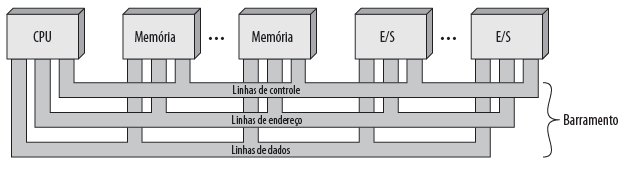
\includegraphics[width=.95\textwidth]{../figs/cap11/barramento.png}
		\end{figure}
		
	\end{frame}
	
	\begin{frame}
		\frametitle{Realização física típica de uma arquitetura de barramento}
		\begin{figure}[hbtp]
		\centering
		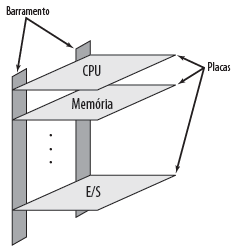
\includegraphics[height=.75\textheight]{../figs/cap11/baramento1.png}
		\end{figure}
		
	\end{frame}
		
	\begin{frame}
		\frametitle{Barramento Local}
		\begin{itemize}
			\item Conexão entre o processador e a memória cache
			\begin{itemize}
				\item Conexão entre cache e memória principal via barramento do sistema
			\end{itemize}
		\end{itemize}
	\end{frame}
	
	\begin{frame}
		\frametitle{Barramento de expansão}
		\begin{itemize}
			\item Conexão de controladores de E/S ao barramento do sistema
			\vspace{1em}
			\item Interface de barramento de expansão
			\begin{itemize}
				\item Isola o tráfego da memória para o processador do tráfego de E/S
			\end{itemize}
		\end{itemize}
	\end{frame}
	
	\begin{frame}
		\frametitle{Arquitetura tradicional}
		\begin{figure}[hbtp]
		\centering
		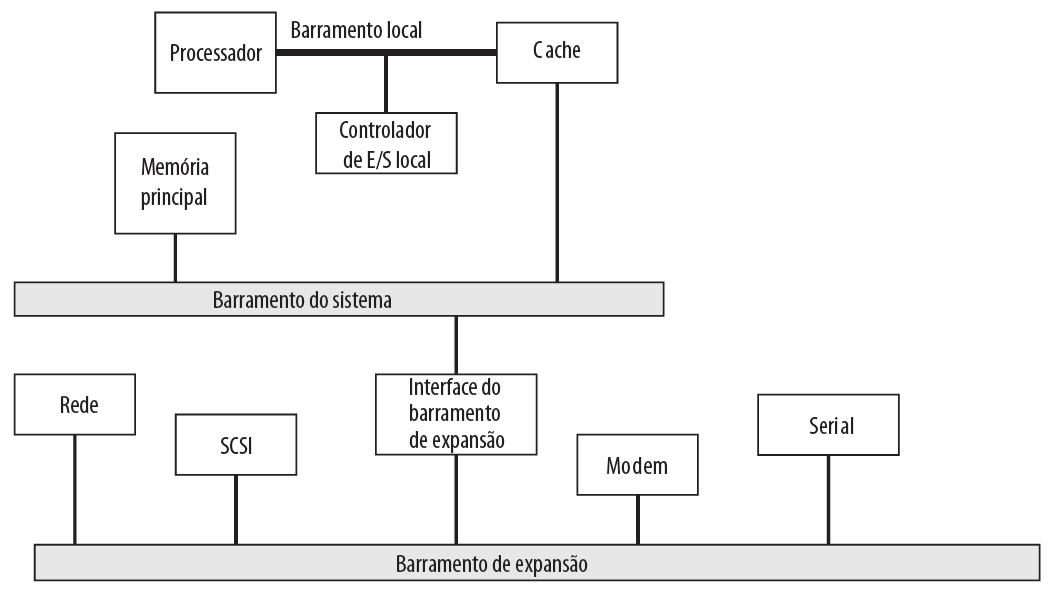
\includegraphics[height=.75\textheight]{../figs/cap11/arquitetura1.png}
		\end{figure}
	\end{frame}
	
	\begin{frame}
		\frametitle{Arquitetura de alto desempenho}
		\begin{figure}[hbtp]
		\centering
		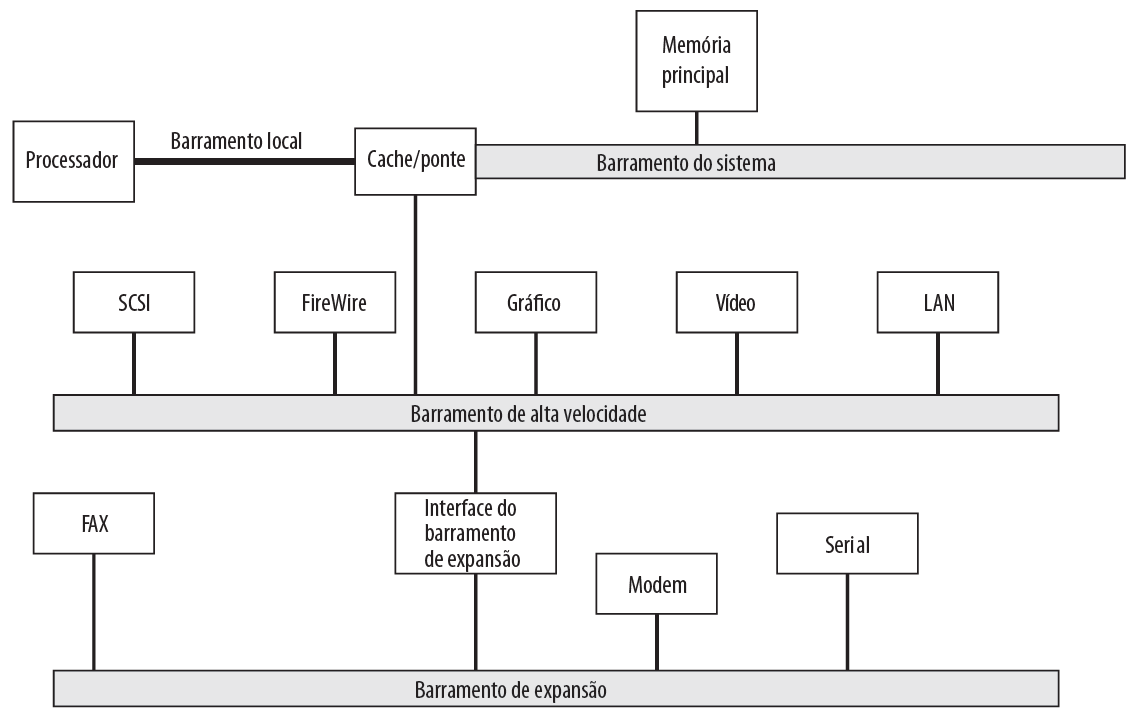
\includegraphics[height=.75\textheight]{../figs/cap11/arquitetura2.png}
		\end{figure}
	\end{frame}		
		
	\section{Projeto do barramento}
	
	\begin{frame}
		\frametitle{Elementos do projeto de barramento}
		\begin{itemize}
			\item Tipos
			\vspace{1em}
			\item Método de arbitração
			\vspace{1em}
			\item Sincronização
			\vspace{1em}
			\item Largura do barramento
			\vspace{1em}
			\item Tipo de transferência de dados
		\end{itemize}
	\end{frame}
	
	\begin{frame}
		\frametitle{Tipos de barramento}
		\begin{itemize}
			\item Dedicada
			\begin{itemize}
				\item Atribuição permanente a uma função ou conjunto de componentes
				\item \textbf{Vantagem:} Alta vazão
				\item \textbf{Desvantagem:} Aumento do tamanho e do  custo do sistema
			\end{itemize}
			\vspace{1em}
			\pause
			\item Multiplexada
			\begin{itemize}
				\item Utilização de uma linha para diversas funções
				\item \textbf{Vantagem:} Economia de espaço e custo
				\item \textbf{Desvantagem:} Circuito mais complexo e redução no desempenho
			\end{itemize}
			
		\end{itemize}
	\end{frame}
	
	\begin{frame}
		\frametitle{Método de arbitração}
		\begin{itemize}
			\item Centralizado 
			\begin{itemize}
				\item Controlador único do barramento. 
				\item Pode ser um módulo específico ou parte do processador.
			\end{itemize}
			\item Distribuído
			\begin{itemize}
				\item Não existe controlador central
				\item Cada módulo contém lógica de controle de acesso
				\item Os módulos atuam juntos para compartilhar o barramento
			\end{itemize}
		\end{itemize}
	\end{frame}
	
	\begin{frame}
		\frametitle{Temporização}
		\begin{itemize}
			\item Modo como os eventos são coordenados no barramento.
			\vspace{1em}
			\item Tipos
			\begin{itemize}
				\item Síncrona
				\item Assíncrona
			\end{itemize}
			
		\end{itemize}
	\end{frame}
	
	\begin{frame}
		\frametitle{Temporização síncrona}
		\begin{figure}[hbtp]
		\centering
		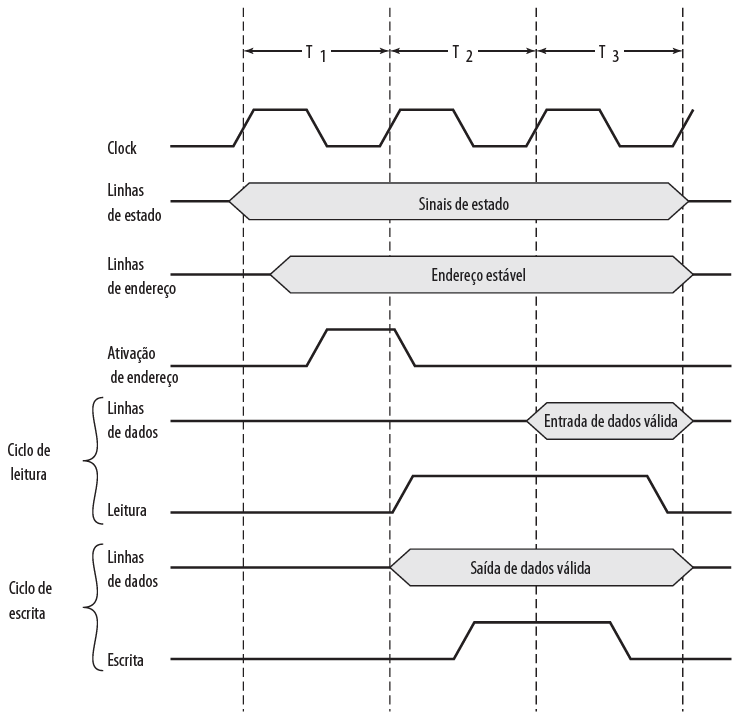
\includegraphics[height=.75\textheight]{../figs/cap11/sincrono.png}
		\end{figure}
	\end{frame}
	
	\begin{frame}
		\frametitle{Temporização assíncrona}
		\begin{figure}[hbtp]
		\centering
		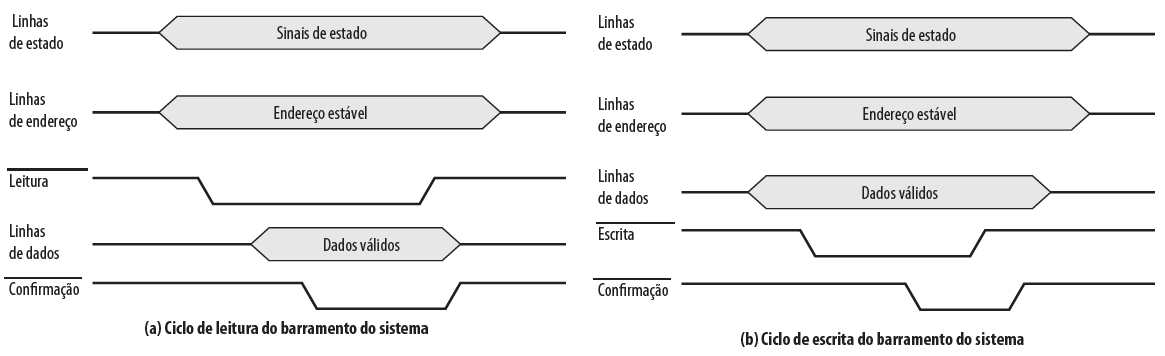
\includegraphics[width=.95\textwidth]{../figs/cap11/assincrono.png}
		\end{figure}
	\end{frame}
	
	\begin{frame}
		\frametitle{Tipos de transferência de dados}
		\begin{itemize}
			\item Leitura
			\vspace{1em}
			\item Escrita
			\vspace{1em}
			\item Ler-modificar-escrever
			\vspace{1em}
			\item Leitura-após-escrita
			\vspace{1em}
			\item Bloco
		\end{itemize}
	\end{frame}
		
	\begin{frame}
		\frametitle{Tipos de transferência de dados}
		\begin{figure}[hbtp]
		\centering
		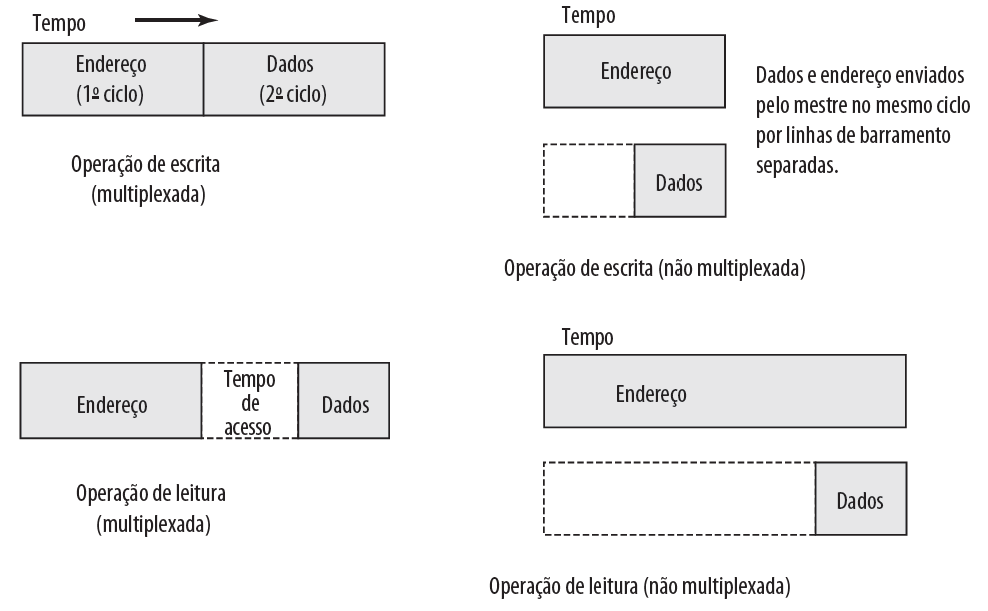
\includegraphics[height=.75\textheight]{../figs/cap11/tipo1.png}
		\end{figure}
	\end{frame}

	\begin{frame}
		\frametitle{Tipos de transferência de dados}
		\begin{figure}[hbtp]
		\centering
		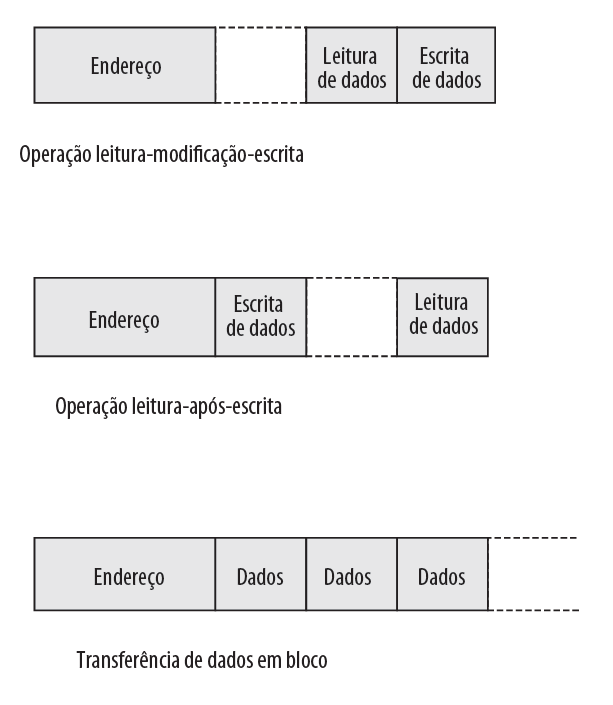
\includegraphics[height=.85\textheight]{../figs/cap11/tipo2.png}
		\end{figure}
	\end{frame}	
	
	\begin{frame}
		\frametitle{Fluxo de Dados}
		
		\begin{itemize}
			\item Simplex
			\begin{itemize}
				\item Comunicação em uma única direção
			\end{itemize}
			\vspace{1em}
			\item Half duplex
			\begin{itemize}
				\item Transmissão e recepção não simultâneas
			\end{itemize}
			\vspace{1em}
			\item Full duplex
			\begin{itemize}
				\item Transmissão e recepção simultâneas
			\end{itemize}
		\end{itemize}
	\end{frame}
	
	\begin{frame}
		\frametitle{Forma de comunicação}
		\begin{itemize}
			\item Serial 
			\begin{itemize}
				\item Um bit por vez
				\item Vias diferentes para transmissão e recepção (\textit{full duplex})
				\item Porta Serial, USB, SATA, \textit{FireWire}
			\end{itemize}
			\vspace{1em}
			\item Paralela
			\begin{itemize}
				\item Cada bit trafega por uma via distinta
				\item Via única para envio e recebimento de dados (\textit{half duplex})
				\item Porta paralela (LPT1), IDE, SCSI, PCI, AGP
				
			\end{itemize}
		\end{itemize}
	\end{frame}
	
	\begin{frame}
		\frametitle{Velocidade Serial \textit{vs.} Paralelo}
		\begin{eftable}

		\begin{tabular}{cc}
		\textcolor{white}{Paralela} & \textcolor{white}{Serial} \\ 
		\textbf{IDE-133:} 133 MB/s & \textbf{SATA III:} 600 MB/s \\ 
		\textbf{LPT:} 300 kB/s & \textbf{USB 2.0:} 480 MB/s \\ 
		\textbf{PCI:} 133 MB/s & \textbf{PCI-Express:} 8 GB/s \\ 
		\end{tabular} 		
		\end{eftable}
	\end{frame}

		
	\section{Categorias}
	
%	\subsection{ISA}
	\begin{frame}
		\frametitle{Barramento ISA}
		\begin{itemize}
			\item \textit{Industry Standard Architeture}
			\vspace{.7em}
			\item Desenvolvido pela IBM em 1981
			\begin{itemize}
				\item Atualmente obsoleto
			\end{itemize}
			\vspace{.7em}
			\item Velocidade: 4.77 MHz ou 8.33 MHz
			\vspace{.7em}
			\item Largura do barramento: 8 ou 16 bits
			\vspace{.7em}
			\item Taxa de transmissão
			\begin{itemize}
				\item Teórica: 8.33 MB/s
				\item Prática: 5 MB/s
			\end{itemize}
		\end{itemize}
	\end{frame}
	
	\begin{frame}
		\frametitle{\textit{Slots} ISA}
		\begin{figure}[hbtp]
		\centering
		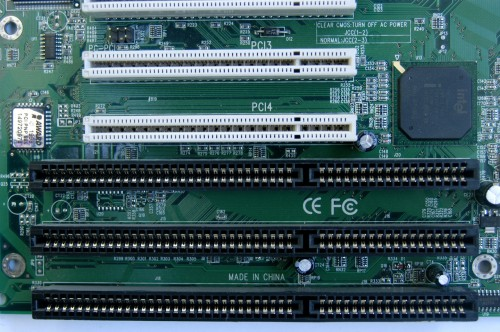
\includegraphics[height=.75\textheight]{../figs/cap11/isa.jpg}
		\end{figure}
	\end{frame}	
	
	\begin{frame}
		\frametitle{Baramento EISA}
		\begin{itemize}
			\item \textit{Extended} ISA
			\vspace{.7em}
			\item Aumento da largura do barramento para 32 bits
			\vspace{.7em}
			\item Compatível com ISA
			\vspace{1em}
			\item Obsoleto desde 1993	
			
		\end{itemize}
	\end{frame}
	
	\begin{frame}
		\frametitle{VESA Local Bus}
		\begin{itemize}
			\item  \textit{Video Electronics Standards Association}
			\vspace{1em}
			\item Extensão do padrão ISA   
			\vspace{1em}
			\item Utilizado inicialmente para vídeo e posteriormente para controladoras IDE e SCSI
			\vspace{1em}
			\item Frequência: 33 MHz 
			\vspace{1em}
			\item Taxa de transferência: até 133 MB/s
		\end{itemize}
	\end{frame}
	
	\begin{frame}
		\frametitle{\textit{Slot} VLB}
		\begin{figure}[hbtp]
		\centering
		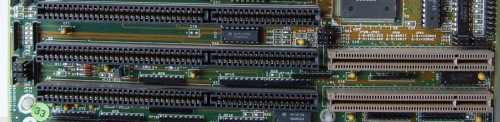
\includegraphics[width=.95\textwidth]{../figs/cap11/vlb.jpg}
		\end{figure}
	\end{frame}	
	
%	\subsection{PCI}
	\begin{frame}
		\frametitle{Barramento PCI}
		\begin{itemize}
			\item \textit{Peripheral Component Interconnect }
			\vspace{1em}
			\item Desenvolvido pela Intel em 1992
			\vspace{1em}
			\item Largura do barramento: 32 ou 64 bits
			\vspace{1em}
			\item Frequência de operação: 33 MHz
			\vspace{1em}
			\item Taxa de transferência: até 132 MB/s		
		\end{itemize}
	\end{frame}
	
	\begin{frame}
		\frametitle{\textit{Bus Mastering}}
		\begin{itemize}
			\item Recurso implementado efetivamente no PCI
			\vspace{1em}
			\item Permite a comunicação direta entre os dispositivos que utilizam o barramento e a memória
			\vspace{1em}
			\item Diminuição do uso do processador
		\end{itemize}
	\end{frame}
	
	\begin{frame}
		\frametitle{\textit{PCI Extended} - PCI-X}
		\begin{itemize}
			\item Evolução do padrão PCI 
			\vspace{1em}
			\item Barramento de 64 bits
			\vspace{1em}
			\item Aumento da frequência de operação: 66, 100, 133 MHz
			\vspace{1em}
			\item Compatível com PCI
		\end{itemize}
	\end{frame}
	
	\begin{frame}
		\frametitle{Conexão de periféricos}
		\begin{figure}[hbtp]
		\centering
		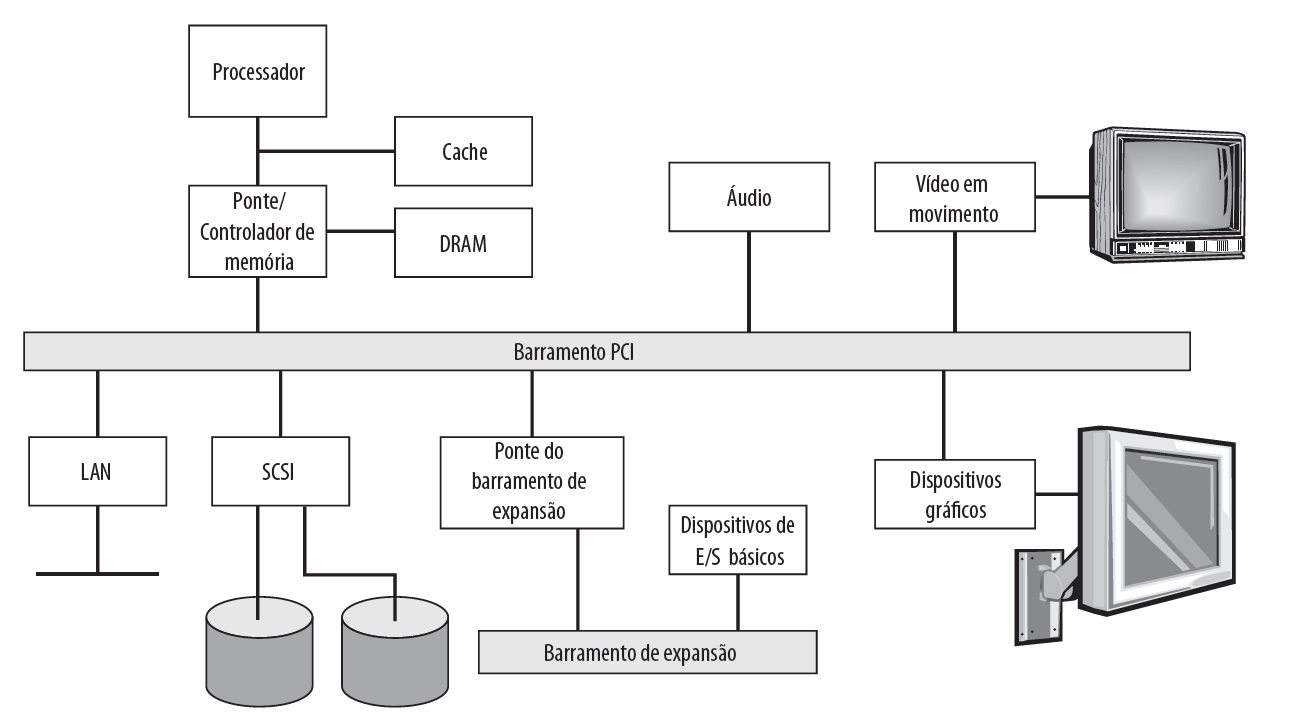
\includegraphics[height=.75\textheight]{../figs/cap11/pci.png}
		\end{figure}
		
	\end{frame}	
	
%	\subsection{AGP}
	\begin{frame}
		\frametitle{Barramento AGP}
		\begin{itemize}
			\item \textit{Accelerated Graphics Port} 
			\vspace{1em}
			\item Lançado pela Intel em 1996 
			\vspace{1em}
			\item Barramento dedicado para vídeo 
			\vspace{1em}
			\item Vantagens
			\begin{itemize}
				\item Operação em capacidade máxima
				\item Utilização da RAM como incremento da memória de vídeo
			\end{itemize}
		\end{itemize}
	\end{frame}
	
	\begin{frame}
		\frametitle{Versões do AGP}
		\begin{eftable}
		\centering
		\begin{tabular}{ccccc}
		{\color[HTML]{FFFFFF} } & {\color[HTML]{FFFFFF} \begin{tabular}[c]{@{}c@{}}Clock\\ (MHz)\end{tabular}} & {\color[HTML]{FFFFFF} \begin{tabular}[c]{@{}c@{}}Largura do\\ barramento\end{tabular}} & {\color[HTML]{FFFFFF} \begin{tabular}[c]{@{}c@{}}Taxa de \\ transferência\end{tabular}} & {\color[HTML]{FFFFFF} Alimentação} \\
		1x & 66 & 32 bits & 266 MBps & 3,3 V \\
		2x &  66 & 32 bits   & 532 MBps & 3,3 V \\
		\multicolumn{1}{l}{4x} &  66 & 32 bits   & 1066 MBps & 1,5 V \\
		\multicolumn{1}{l}{8x} &  66 & 32 bits   & 2133 MBps & 0,8 V
		\end{tabular}
		\end{eftable}		
	\end{frame}
	
%	\subsection{PCI Express}
	\begin{frame}
		\frametitle{Barramento PCI Express}
		\begin{itemize}
			\item Desenvolvido pelo grupo Intel/Dell/HP/IBM em 2004
			\vspace{1em}
			\item Substitui os padrões PCI e AGP
			\vspace{1em}
			\item Barramento \alert{serial dedicado}
			\vspace{1em}
			\item Alta velocidade
			\vspace{1em}
			\item \textit{Hot plug}
		\end{itemize}
	\end{frame}
	
	\begin{frame}
		\frametitle{Versões do AGP}
		\begin{eftable}
		\centering
		\begin{tabular}{ccc}
		{\color[HTML]{FFFFFF} } &
		{\color[HTML]{FFFFFF} \begin{tabular}[c]{@{}c@{}}Clock\\ (GHz)\end{tabular}} &
		{\color[HTML]{FFFFFF} \begin{tabular}[c]{@{}c@{}}Taxa de \\ transferência\end{tabular}} \\
		1.0 & 2.5 & 250 MBps \\
		2.0 & 5.0 & 500 MBps \\
		3.0 & 8.0 & 1000 MBps \\
		\end{tabular}
		\end{eftable}	
	\end{frame}
	
%	\subsection{USB}
	\begin{frame}
		\frametitle{\textit{Universal Serial Bus} - USB}
		\begin{itemize}
			\item Lançado em 1996
			\vspace{1em}
			\item \textit{Hot plug}
			\vspace{1em}
			\item \textit{Plug and play}
			\vspace{1em}			
			\item Facilidade de conexão de novos periféricos
			\vspace{1em}
			\item Expansibilidade (até 127 dispositivos)
		\end{itemize}
	\end{frame}
	
	\begin{frame}
		\frametitle{Conexão de periféricos}
		\begin{figure}[hbtp]
		\centering
		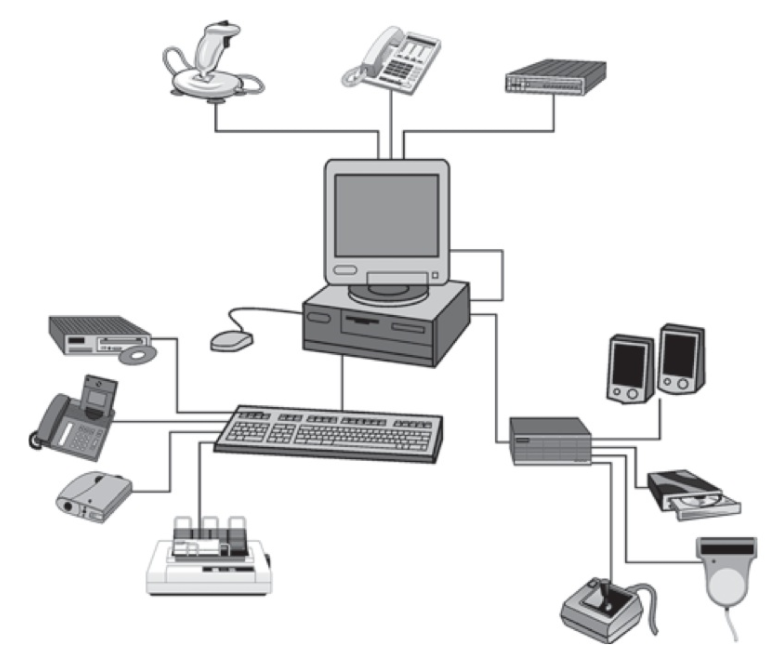
\includegraphics[height=.75\textheight]{../figs/cap11/usb.png}
		\end{figure}
		
	\end{frame}
	
	\begin{frame}
		\frametitle{Versões}
		\begin{itemize}
			\item USB 1.1
			\begin{itemize}
				\item Lançada em 1996
				\item Velocidade: 12 MBps
			\end{itemize}
			\vspace{1em}
			\item USB 2.0
			\begin{itemize}
				\item Lançada em 2002
				\item Velocidade: 60 MBps
			\end{itemize}
			\vspace{1em}
			\item USB 3.0
			\begin{itemize}
				\item Lançada em 2009
				\item Velocidade: 600 MBps
			\end{itemize}
		\end{itemize}
	\end{frame}

	\section{Exercicios}
	
	\begin{frame}{Questão 1 - CFO-DF 2017}
		Todos os barramentos possuem a mesma estrutura, sendo classificados em dois grupos funcionais: linhas de dados e endereço.

	\end{frame}

	\begin{frame}{Questão 2 - CFO-DF 2017}

		Em um barramento, se dois dispositivos transmitirem durante o mesmo período, seus sinais serão sobrepostos e ficarão distorcidos.

	\end{frame}
	
	\begin{frame}{Questão 3 - CEGÁS 2017}
		Assinale a única alternativa que corresponde a seguinte definição: “É o padrão de barramento externo ao computador, esta tecnologia tornou mais fácil a tarefa de conectar aparelhos e dispositivos periféricos (como teclados, mouse, modems, câmeras digitais) sem a necessidade de desligar/reiniciar o computador (“Plug and Play”) e com um formato diferenciado, universal, dispensando o uso de um tipo de conector específico para cada dispositivo.”: 
		\begin{enumerate}[a]
			\item Interface SCSI.
			\item Interface USB.
			\item Interface serial. 
			\item Interface paralela. 
		
		\end{enumerate}
	\end{frame}
	
	
	\begin{frame}{Questão 4 - UFPA 2017}
		Sobre o barramento PCI-Express 16x, é CORRETO afirmar que 
	
		\begin{enumerate}
			\item é geralmente utilizado para transmissão de dados de rede no computador para melhorar a velocidade da conexão com a Internet.  
	  
			\item substitui completamente os antigos padrões (AGP e PCI) nos computadores modernos, por ser mais barato. 
	  
			\item é geralmente utilizado em uma placa de vídeo dedicada, melhorando o desempenho dos softwares que dependem de renderização gráfica. 
	  
			\item é uma versão melhorada do barramento PCI, sendo assim, utilizado para conexão de vários periféricos de entrada e saída (interfaces humano computador), melhorando o desempenho do computador. 
	  
			\item é exclusivo para conexão com o chipset do computador, uma vez que há necessidade de troca rápida de informação entre os componentes do computador. 
		
		\end{enumerate}

	\end{frame}
	
	\begin{frame}{Questão 5 - FUB 2016}
		Em um sistema de computação, o barramento de dados é bidirecional e o barramento de endereços é unidirecional.

	\end{frame}
	
	\begin{frame}{Questão 6 - TCE-PA 2016}
		Nos computadores pessoais, os barramentos internos ao microprocessador interligam os registradores, caches internos e demais componentes do processador, ao passo que os barramentos locais conectam placas controladoras, interfaces e periféricos.

	\end{frame}
	
	\begin{frame}{Questão 7 - BAHIAGÁS 2016}
		Os computadores pessoais, desktops, costumam possuir “slots” ou barramentos de expansão. Sobre estes “slots”, marque a alternativa correta:
		\begin{enumerate}[I]
			\item O slot AGP (Accelerated Graphics Port) foi um barramento de alta velocidade desenvolvido para integrar, originalmente, placas de vídeo 3D de alto desempenho.
			\item O barramento ISA (Industry Standard Acrchitecture) suporta frequências mais altas que o barramento PCI (Peripheral Component Interconnect).
			\item O barramento PCIe (PCI express) é um barramento de alta velocidade desenvolvido exclusivamente para placas ethernet com suporte ao padrão gigabit.
			\item O barramento PCIe (PCI express) é uma extensão do PCI que suporta frequência máxima de 66MHz.
Em relação a estas afirmações, assinale a alternativa correta: 
		
		\end{enumerate}

	\end{frame}
	
	\begin{frame}{Questão 8 - Telebras 2015}
		Se um barramento de dados tiver mais de uma CPU, uma das soluções para evitar a inconsistência das operações é adotar o ciclo de barramento ler–modificar–escrever.

	\end{frame}
	
	\begin{frame}{Questão 9 - UFPA 2015}
		O controlador de barramento é um chip cuja função no computador é
		\begin{enumerate}[a]
			\item verificar as requisições de acesso ao barramento, intercalando requisições de E/S com requisições de CPU.
  
			\item decidir quem deve utilizar o barramento do computador, este sempre dá prioridade para os dispositivos E/S em detrimento da CPU.
  
			\item verificar a temperatura do barramento. Sempre que o barramento esquenta mais do que o permitido, o árbitro de barramento interrompe a utilização deste, para evitar danos ao computador.
  
  			\item decidir quais dados vão trafegar no barramento para controle de segurança dos dispositivos.
  
  			\item dividir o barramento para sua utilização em paralelo, por dois ou mais dispositivos.
		
		\end{enumerate}
	\end{frame}

	\section{Referências}
	\begin{frame}{Bibliografia}
		\nocite{Delgado2017}
		\nocite{Stallings2010}
    	\bibliographystyle{ieeetr}
    	\bibliography{../refs}   	
	
	\end{frame}

\end{document}